\pagestyle{fancy}
\normalsize
\linespread{1.5}\selectfont
\chapter{绪论}
\addtocontents{los}{\protect\addvspace{10pt}}

\section{研究背景}
领域特定语言的研究及应用日益广泛,其中不乏正则表达式、SQL、XML等应用场合及其多的领域特定语言。而随着计算机科学技术的发展,更多新颖的的场景(引用)加入到了使用DSL的队伍。而在一般场合中,语言设计者是计算机科学家,语言使用者却是领域内的专家。因此,当领域特定语言的使用出现一些问题时,领域内的专家(使用者)需要得到领域特定的信息来进行处理。

语法糖是近些年一种流行的领域特定语言实现方法,其方法源于Lisp的宏系统(Macro),经过Scheme语言的发展,再到Racket语言的扩展。(可以引用From …那篇的部分)语法糖构造DSL的最主要优点就是简单高效,语言设计者只需要写一个简单的映射,就可以构造DSL。

然而,语法糖的一项缺陷,导致其应用领域一直局限于计算机科学内部。我们先来看下面这个例子。
\begin{quote}
	(举一个开药方/饭店流程的例子)
\end{quote}

%将这个例子抽象到简单的例子and(or(1,0),and(1,0))

我们可以看到,在执行过程中,语法糖被展开成if,在通用语言中继续执行,得到最终结果。但实际应用到特定领域时,我们很明显不希望得到这样复杂的执行过程,特别是对于对计算机内部语言不熟悉的领域专家来说,这种执行过程是没有意义的。

\section{解决的问题及研究现状}
我们将上述问题总结为语法糖解糖的单向性,对上面的例子的xx行todo,我们可以看出,其存在等价的领域特定语言表示and(1,and(1,0))。如果语法糖的解糖有一个逆过程(重组糖),我们就可以找到其对应的这样一个序列。我们将在第二章对问题进行形式化定义。我们在后文,将领域特定语言视为外部语言,通用语言视为内部语言。

\section{相关工作及存在的问题}
我们的方法主要借鉴和对比Resugaring系列一些工作,其中前两篇和本文的工作紧密相关,我们将简单讲述一下这两篇工作的方法及缺陷

第一篇介绍的方法,基本思想是将内部语言的求值序列每一步加上标签,进行搜索,试图得到其对应的在外部语言的表示。

其算法希望具有如下三个性质:

仿真性/抽象性/覆盖性(没有被证明)

第二篇工作在第一篇的基础上,新增了两个优点:1.解决卫生宏 2.拓展语法糖规则(超过syntax-rule)3.覆盖性得到形式化证明

然而该工作仍然存在一些问题:

1.	语法糖规则依然不够丰富

2.	算法定义繁琐,通用性差。
\section{基本思路及全文结构}

本文基于语义工程工具PLT Redex,设计了一个全新的语法糖——重组糖框架。其想法源于完全β规约的完备性,如下图。

\begin{figure}[h]
	\centering
	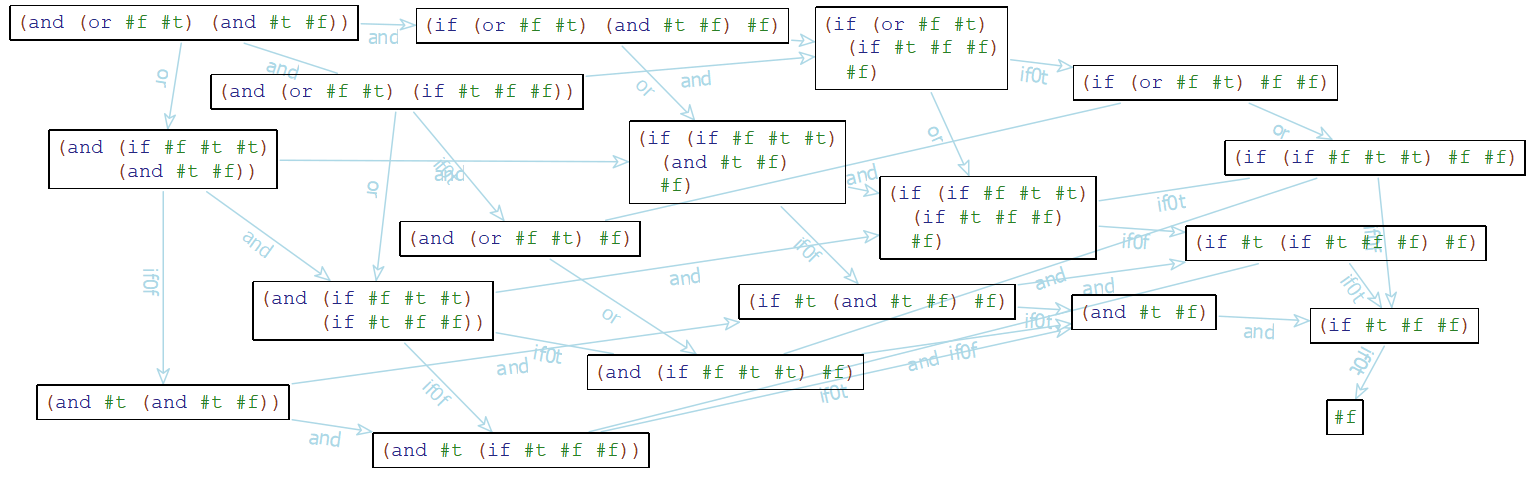
\includegraphics[width=12cm]{images/chapter1/example.png}
	\caption{基本思路}
\end{figure}

该例子中,对一个结构化(类似S表达式,定义在第二章)的语言,定义其基础语义和规约规则。其中and和or是语法糖,语法糖展开内部语言的if表达式。在没有限制其上下文规则(求值顺序)的前提下,生成了其规约的流程图。我们可以看出,在该图中,既包含了将语法糖展开的规约,也包含了我们期待的and()等等这些中间求值路径。因此我们希望使用基于规约语义的PLT Redex,实现一个轻量级的重组糖,在这个完全图中提取出我们需要的重组糖序列。

在实现过程中,我们发现生成中国完全图并不是必须的,而我们可以在从最初的表达式开始{\bfseries 每次进行单步规约,在一条或多条规约规则中选择我们需要的那条规约规则 }(是本工作的核心算法),且该规则的多次执行保证重组糖的三个基本重要性质。则在这个核心算法迭代执行过程中,会留下一个对应的求值序列,在其中提取出符合输出规则的中间序列,则此序列即为重组糖的输出。

我们将在第二章讲述本文工作的一些背景知识及思考路线,第三章讲述工作的算法定义及正确性证明,第四章讲述一些实现算法的具体细节及对一些语法糖例子进行讨论评估,第五章总结我们的工作,并对一些未来可能的方向进行简单探讨与展望。

\section{本文主要贡献}
\begin{flushleft}
	1.	我们针对现有重组糖的方法法进行改进,得到新的轻量级重组糖方法。
\end{flushleft}

\begin{itemize}
	\item 我们的方法不需要将所有语法糖都展开就可以得到重组糖序列,而现有方法需要展开后在内部语言执行,并基于match和substitute对可重组的语法糖进行搜索。
	\item 我们的方法处理卫生宏很简单而自然,而现有工作处理卫生宏需要引入新的数据结构以及很多其他处理。
\end{itemize}
\begin{flushleft}
	2.	我们的方法相对于现有重组糖方法,支持更多语法糖特性。
\end{flushleft}

\begin{itemize}
	\item 对递归糖,我们的方法可以很简单的处理。而现有方法只能用letrec处理一下递归绑定。
	\item 对高阶糖,我们的方法也可以很容易处理。而现有方法不能处理。
\end{itemize}
\begin{flushleft}
	3.	我们的轻量级重组糖算法在对领域特定语言的解释器进行自动生成的研究提供了一个思路。我们将在未来工作中进一步讨论。
\end{flushleft}



